\newpage

\section{Luminosity functions}
One of the most effective methods for quantifying galaxy evolution over cosmic time is with the luminosity function (\gls{lf}). Luminosity functions are statistical distributions that describe the spatial density of astronomical objects at various luminosities and redshifts, and so are a fundamental tool for quantifying their evolution across cosmic time \citep{han_evolution_2012, dai_mid-infrared_2009, wylezalek_galaxy_2014}. In this section, I focus on and give a review of \gls{ir} \gls{lf}s and provide a brief overview of other wavelengths. In \cref{Sec: Luminosity Functions Chapter}, I will introduce how to calculate \gls{lf}s and show the results of preliminary tests. 

\begin{figure}[h!]
    \centering
    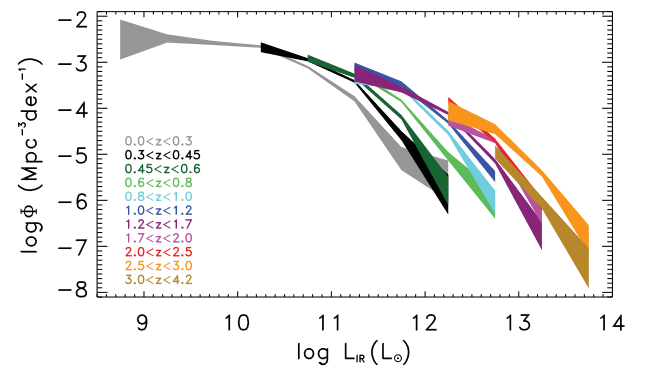
\includegraphics[width=\linewidth]{Figures/grupp_LF.png}
    \caption{The total IR LF across various redshift bins from \cite{gruppioni_herschel_2013} using the \textit{Herscel} Space Telescope. Number densities ($\phi$) are colour-filled between the uncertainty bounds. Each colour represents a separate redshift bin, with $0.0<z<0.3$ being the LF of the local universe and $3.0<z<4.2$ being 11.64 to 12.34 Gyrs ago, respectively. The number density evolution is represented across 90\% of the universe's existence. Credit: C. Gruppioni, Figure 8, © MNRAS, 432, 23–52.}
    \label{Fig: Example LF Gruppioni}
\end{figure}

\Cref{Fig: Example LF Gruppioni} shows the \gls{lf}s calculated by \citep{gruppioni_herschel_2013}. This is an example \gls{lf} plot and represents the combined redshift evolution. It can be seen that, at fixed IR luminosity, the number density of galaxies decreases with decreasing redshift from $z\approx 2$. This is a tentative discovery of a \textit{downsizing} effect, whereby the brightest galaxies decline in number density faster at higher redshift than fainter luminosity counterpart galaxies. This is reinforced by the fact that galaxies above $z>2$ appear to increase in number density with increasing luminosity and redshift and decrease in number density from $z\approx2.5$ onwards. This coincides within the peak of cosmic \gls{sf} rate history \citep{madau_cosmic_2014}.

Analysing the simple number density distribution of galaxies and how they evolve with redshift can yield a surprising amount of information about the general evolution of the universe. However, \cite{gruppioni_herschel_2013} does not perform \gls{sed} decomposition to separate the \gls{agn} component to the \gls{lf}. As highlighted in the previous \cref{Sec: Spectral Energy Distributions}, essential discoveries concerning the co-evolution of galaxies and \gls{agn} are to be made by analysing the simultaneous evolution of \gls{agn} with their host galaxy and \gls{sf}. 

\subsection{Malmquist Bias}

\begin{figure}[h!]
    \centering
    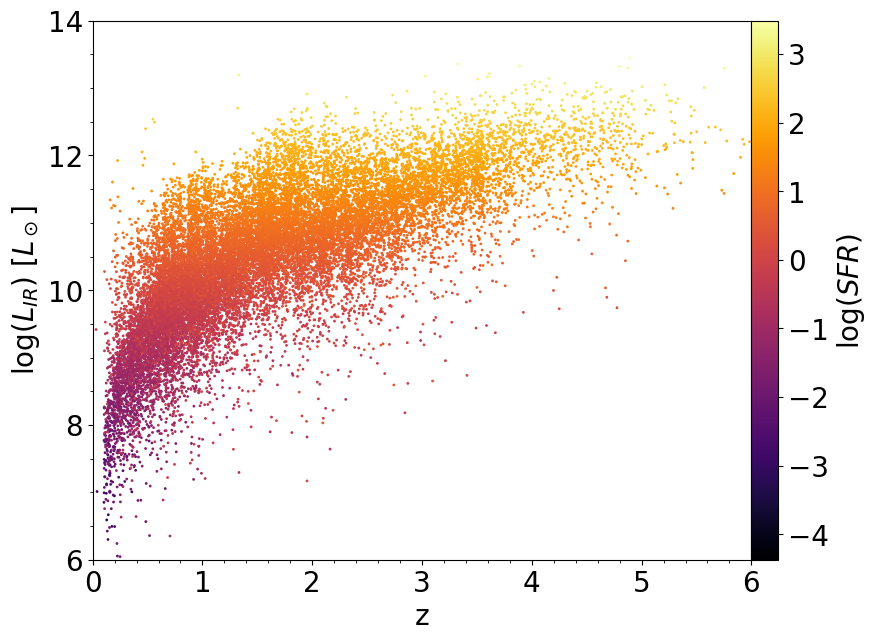
\includegraphics[width=\textwidth]{Figures/ZFOURGE Initial Distribution.png}
    \caption{The distribution of ZFOURGE galaxies used in this thesis. Galaxies are coloured based on their SFR, which is derived by the \cite{kennicutt_global_1998} scaling factor of the total IR luminosity. This figure does not highlight galaxies that may or may not be later removed in data reduction. Malmquist bias is evident: only the largest galaxies at higher redshifts are identified.}
    \label{Fig: ZFOURGE Distribution}
\end{figure}

\Cref{Fig: ZFOURGE Distribution} illustrates the relationship between luminosity and redshift for all sources in \gls{zfourge} \citep{straatman_fourstar_2016}. A prominent feature is the presence of Malmquist bias \citep{malmquist_relations_1922}, a selection effect whereby the most distant objects are also among the brightest observed. This bias arises simply due to the inverse square law: intrinsically bright objects can be detected further than intrinsically faint objects. When observations are conducted, telescopes are pointed at a specific region in space and data is collected over a predetermined exposure time. For an astronomical object to be detected by any telescope, it must meet a minimum threshold of brightness or distance. This is known as the flux limit and is defined by the quantity of energy received by the area of a telescope's mirrors over a specified duration (measured in $J \ m^{-2} \ s^{-1}$). The flux limit is primarily influenced by the observing instrument's sensitivity, aperture size, and exposure time, which determine the faintest objects that can be detected in a survey.

To observe the most distant and faint objects, it is essential to develop more sensitive telescopes, such as the recently operational \gls{jwst} \citep{gardner_james_2006}, which offers unprecedented sensitivity and resolving power in the \gls{ir} \citep{labiano_wavelength_2021}. Additionally, the Square Kilometer Array \citep{dewdney_square_2009} represents a next-generation radio telescope capable of identifying intermediate-redshift ($z<2$) radio galaxies through their neutral hydrogen content, the most prevalent element in the early universe \citep{furlanetto_cosmology_2006}.

By studying the simple distribution of galaxies --- the number of galaxies per unit volume of space through cosmic time --- we can observe how the \gls{lss} of the universe has changed and begin to understand how various types of galaxies have influenced that evolution. The most direct method of measuring the distribution of galaxies is with the \gls{lf}. The effect of Malmquist bias is effectively minimised in \gls{lf}s because number density corrects for the difference in the volume over which galaxies of different luminosities are observable. By expressing the count of galaxies as a function of volume and luminosity, it provides a more accurate representation of the intrinsic galaxy population. How this is achieved in practice is explained in \cref{Sec: Luminosity Functions Chapter}.